\documentclass{report}
\usepackage[pdftex]{graphicx}
\usepackage{sidecap}
\usepackage{fancyhdr}
\usepackage{lscape}
\usepackage[francais]{babel} 
\usepackage[absolute]{textpos}
\usepackage{amssymb}
\usepackage{siunitx}

\usepackage[utf8]{inputenc}  
\usepackage[T1]{fontenc}


\title{Rapport de labo d'\'electronique: \\ Semi-conducteurs, diodes et transistors}
\author{Groupe ?: \\ Mattens Simon; Dom Eduardo \\ BA2 Info}
\date{Labo r\'ealis\'e le 26 avril 2018}

\pagestyle{fancy}
\lhead{Groupe ?: Mattens S. ; Dom E.}
\rhead{BA2 Info}
\cfoot{\thepage}
\begin{document}
\maketitle


\section*{1. Introduction}
Le but de la manipulation est l'étude des caractéristiques électriques d'une diode à semi-conducteur, d'une diode Zener ainsi que d'un transistor bipolaire à jonctions.

\section*{2. R\'esum\'e th\'eorie}
\begin{itemize}
\item Les semi-conducteurs ont une résistivité électrique intermédiaire entre celle des isolants et celle des conducteurs. Les plus connus sont le germanium(Ge) et le silicium(Si) qui sont les constituants de base des diodes de cristal.
\item A température ambiante, il peut se faire qu'un électron possédant assez d'énergie quitte sa place. L'électron est libre de se mouvoir et sa place devenue libre est appellée trou.
\item Pour augmenter la conductivité, il faudrait pouvoir augmenter soit le nombre d'électrons, soit le nombre de trous. On y arrive en injectant des "impuretés" dans le cristal de semi-conducteur pur.
\item Un cristal de Ge contenant des atomes accepteurs est dit du type p si il possède des ions négatifs fixes et des trous libres.
\item Un critsal de Ge contenant des atomes donneurs et dit de type n si il possède des ions positifs fixes et des électrons libres.
\item Quand on accole un cristal de semi-conducteur de type p et un cristal de type n, la surface de contact entre les deux cristaux s\ 'appelle jonction p-n. Il apparaît au voisinage de la jonction une différence de potentiel de contact et donc un champ électrique s'opposant petit à petit à la diffusion des charges mobiles.
\item Aucun courant ne circule dans le cristal lorsqu'on polarise le cristal p ! n en appliquant une différence de potentiel de même sens que la différence de potentiel de contact.(Sens bloquant, exprimé généralement en nA).
\item Lorsqu'on polarise le cristal p! n en appliquant une différence de potentiel de sens contraire de la différence de potentiel de contact un courant circule dans le circuit.(Sens passant, exprimé en mA).
\item Le transistor bipolaire à jonction est constitué d'un monocristal comprenant 3 régions : 2 régions p séparées par une région n ou 2 régions n séparées par une région p. On parle alors de transistor p-n-p ou de transistor n-p-n.On appelle base la région commune p (ou n), émetteur la région n(ou p) de la diode 1 et collecteur la région n(ou p) de la diode 2.
\newpage
\textbf{Transistor bipolaire à jonction : }
\begin{figure}[h!]
\centering
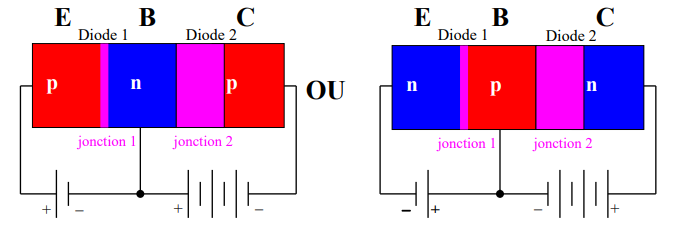
\includegraphics[scale=0.5]{Trans.png}
\end{figure}
\\
\textbf{Symbole d'une diode : }
\begin{figure}[h!]
\centering
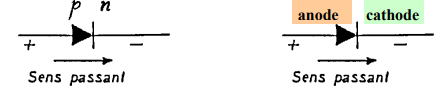
\includegraphics[scale=0.5]{Diode.png}
\end{figure}
\\
\textbf{Transistor pnp : }
\begin{figure}[h!]
\centering
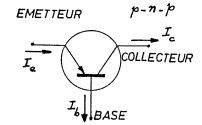
\includegraphics[scale=1]{pnp.png}
\end{figure}
\\
\textbf{Transistor npn : }
\begin{figure}[h!]
\centering
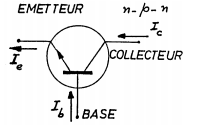
\includegraphics[scale=1]{npn.png}
\end{figure}

\end{itemize}

\newpage

\section*{3 Dispositif exp\'erimental}

\subsection*{3.2 Relevé de la courbe I = f(U) d'une diode à jonction}

\subsubsection*{3.2.1 Circuit de polarisation en sens bloquant de la diode}
Nous avons r\'ealis\'e le circuit repr\'esent\'e par le sch\'ema suivant :\\

\textbf{Sch\'ema de l'exp\'erience: }
\begin{figure}[h!]
\centering
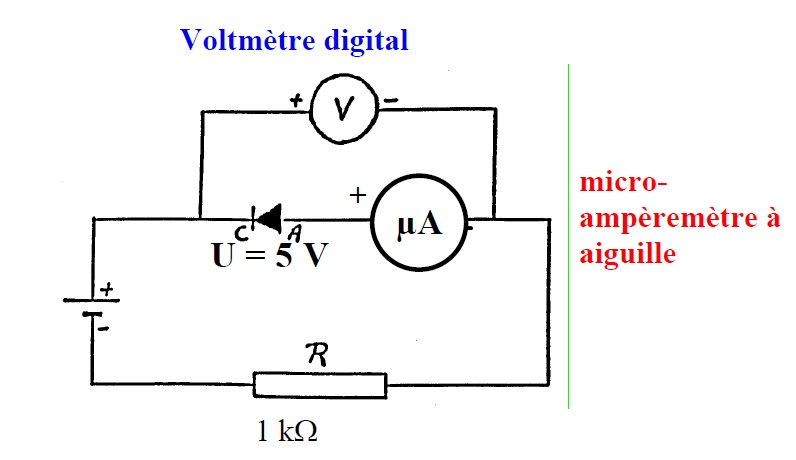
\includegraphics[scale=0.5]{ScheBlo.jpg}
\end{figure}

\newpage
\subsubsection*{3.2.2 Circuit de polarisation en sens passant de la diode}

Nous avons réalisé le circuit représenté par le schéma suivant :\\

\textbf{Schéma de l'expérience: }
\begin{figure}[h!]
\centering
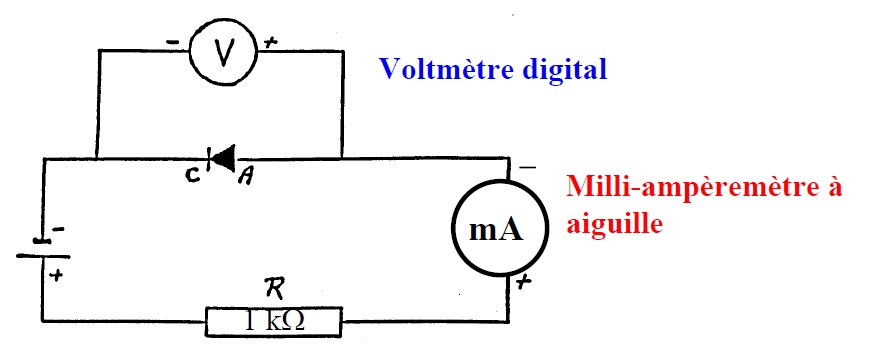
\includegraphics[scale=0.5]{SchePas.jpg}
\end{figure}
\newpage

\subsubsection*{3.2.3 Observation de la courbe à l'oscilloscope}
Nous avons réalisé le circuit représenté par le schéma suivant : \\

\textbf{Schéma de l'expérience: }
\begin{figure}[h!]
\centering
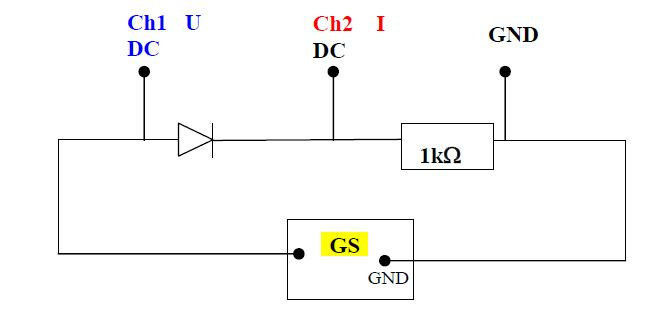
\includegraphics[scale=0.5]{ScheOs.jpg}
\end{figure} \\

\subsection*{3.4 Diodes LED : observations à l'oscillo}
Nous avons réalisé le circuit représenté par le schéma suivant : \\

\textbf{Schéma de l'expérience: }
\begin{figure}[h!]
\centering
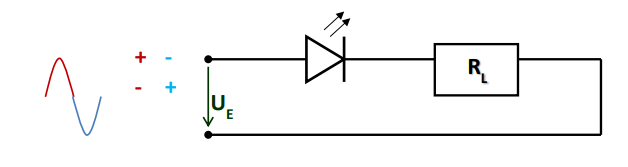
\includegraphics[scale=0.5]{led.png}
\end{figure} \\

\subsection*{3.5 Etude qualitative d'un transistor bipolaire : 2 jonctions}

\begin{itemize}
\item 2N3546 : p-n-p
\item 2N1711: n-p-n
\end{itemize}
\newpage

\subsection*{3.6 Mesures de tensions et courants}
Nous avons réalisé le circuit représenté par le schéma suivant : \\

\textbf{Schéma de l'expérience: }
\begin{figure}[h!]
\centering
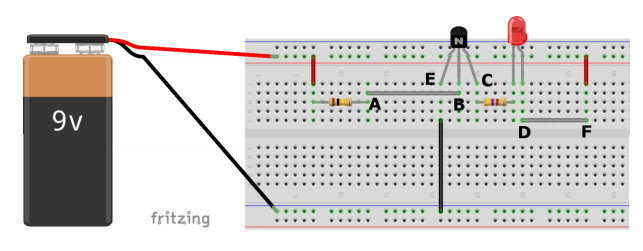
\includegraphics[scale=0.5]{schema.png}
\end{figure} \\

\subsection*{3.7 Principe d'utilisation d'un transistor BJT(ou FET) comme switch ou interrupteur}
Il nous ait demandé de vérifier le mode de fonctionnement "commutateur" du transsitor bipolaire sur le circuit suivant :\\
\textbf{Schéma de l'expérience: }
\begin{figure}[h!]
\centering
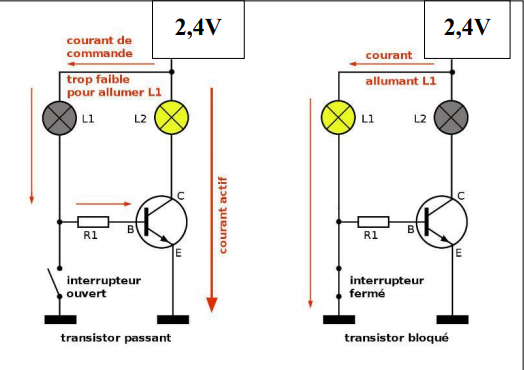
\includegraphics[scale=0.5]{end.png}
\end{figure} \\
\newpage
\section*{4 Prise des mesures et résultats}


\subsection*{4.1 Relevé de la courbe I = f(U) de la diode}

\subsubsection*{4.1.1 Circuit de polarisation en sens bloquant de la diode}

\textbf{\'Enonc\'e:} Mesurer la résistance ohmique de la diode en utilisant la fonction prévue à cet effet au multimètre \\

\textbf{R\'eponse:}
\begin{itemize}
\item Sens direct : 0,643k$\si{\ohm}$
\item Sens bloquant : 1k$\si{\ohm}$ 
\end{itemize}

Nous avons remarqué qu'aucun courant n'est mesurable par le micro-ampèremètre.

\subsubsection*{4.1.2 Circuit de polarisation en sens passant de la diode}

Nous avons mesuré le potentiel du circuit et l'intensité du courant passant dans la diode selon le potentiel de la diode. Voici ces mesures sous forme de tableau.\\

\begin{tabular}{|c|c|c|}
\hline
\textbf{U circuit(V)} & \textbf{U diode(V)} & \textbf{I  diode(mA)} \\
\hline
0,5 & \textbf{0,50V} & 0,03  \\
\hline
0,7 & \textbf{0,55V} & 0,12 \\
\hline
1,0 & \textbf{0,60V} & 0,41 \\
\hline
1,5 & \textbf{0,65V} & 0,82 \\
\hline
3 & \textbf{0,70V} & 2,31 \\
\hline
6,4 & \textbf{0,75V} & 5,66 \\
\hline
12,5 & \textbf{0,80V} & 11,70  \\
\hline
25,2 & \textbf{0,85V} & 24,4\\
\hline
\end{tabular}
\newpage
Voici le graphique de la variation de U circuit en fonction de U diode:
\begin{figure}[h!]
\centering
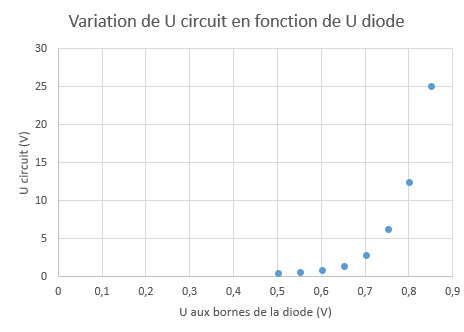
\includegraphics[scale=0.75]{UU.png}
\end{figure}
\\
Voici le graphique de la variation de I en fonction de U diode:
\begin{figure}[h!]
\centering
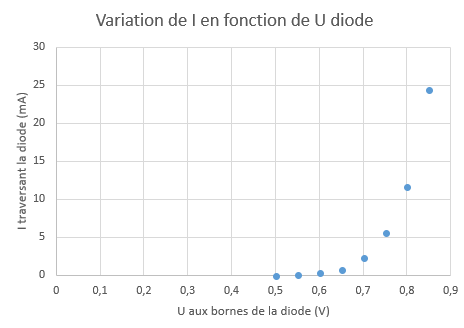
\includegraphics[scale=0.75]{UI.png}
\end{figure}

\newpage
\subsubsection*{4.2 Observation de la courbe \`a l'oscilloscope}
Pour visualiser les variations du courant I, on visualise les variations de la tension $U_{R}$ aux bornes d'une résistance R placée en série dans le circuit.\\

\textbf{\'Enonc\'e:} Cette tension est proportionnelle au courant I. Pourquoi ?\\

\textbf{R\'eponse:} \\

Parce que $U_{R} = R_{R} \cdot I_{R}$, on a donc que $U_{R}$ est directement proportionnel au courant passant dans la résistance.\\


Les conditions pour le générateur de tension étaient les suivantes : 

\begin{itemize}
\item Fr\'equence du signal sinusoidal : 380Hz
\item Amplitude du signal : 1,5V
\end{itemize}

\subparagraph*{4.2.1 Première observation} ~~\\

\begin{figure}[h!]
\centering
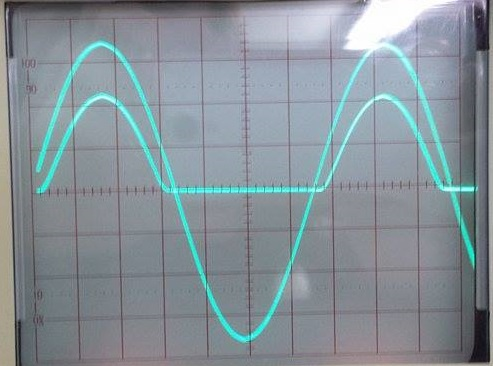
\includegraphics[scale=0.65]{Oscillo.jpg}
\end{figure}

\pagebreak

\subparagraph*{4.2.2 Observation en mode 'Lissajous'} ~~\\

\begin{figure}[h!]
\centering
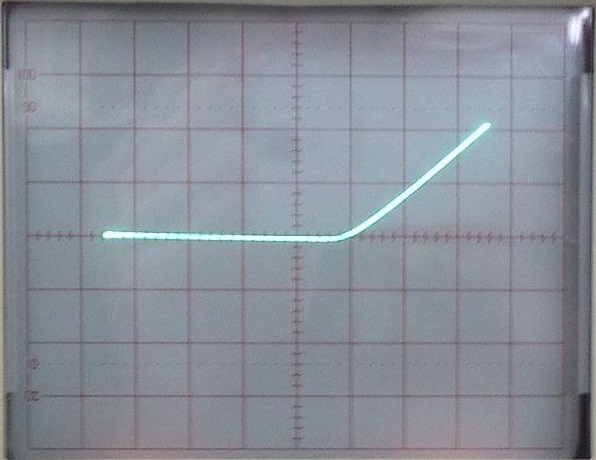
\includegraphics[scale=0.5]{Lissajou.jpg}
\end{figure}
Nous remarquons qu'il n'y a pas de courant quand U est négatif, celui-ci démarre lorsque U atteint les 400mV et le courant devient nul bien avant que la tension ne le soit.
\\ La tension seuil avant que le courant puisse passer est de l'ordre de 400mV.

\subsubsection*{4.3 Diode Zener}

\textbf{\'Enonc\'e:} Mesurer la résistance ohmique de la diode Zener \\

\textbf{R\'eponse:} 

\begin{itemize}
\item sens passant : 0,712k$\si{\ohm}$
\item sens bloquant: 1k$\si{\ohm}$
\end{itemize}

Avec la diode Zener nous observons qu'à partir de 5,1V la diode laisse passer le courant, lorsque la tension est négative le courant arrive quand même à passer et n'est plus nul.

\subsubsection*{4.4 Diodes LED}
Au plus la fréquence est basse au plus la diode LED va clignoter de plus en plus lentement.
Nous imaginons que lorsque la fréquence est à 200Hz, notre oeil ne peut pas suivre les clignotements de la LED tellement ceux-ci sont rapides.

\subsubsection*{4.6 Mesures de tensions et courants}

\begin{itemize}
\item Mesure de la tension entre émetteur et base : 0,65V
\item Mesure de la tension entre émetteur et collecteur : 6,80V
\item Mesure de la tension entre base et collecteur : 6,47V
\item La tension attendue entre ces tensions est exacte car 6,80$\simeq$ 0,65+6,47 (Ie=Ic+Ib).
\item Lorsqu'on enlève le fil entre A et B et qu'on met notre pouce sur A et l'index sur B la LED s'allume.
\item 84,8mA
\item 2,56mA
\item le gain du transistor est de : ?
\end{itemize}

\section*{5 Analyse des résultats}

\subsection*{5.1 Relev\'e de la courbe I = f(U) de la diode}

\subsubsection*{5.1.1 Circuit de polarisation en sens bloquant de la diode}

Nous avons essayé de mesurer un courant passant par la diode avec un micro-amp\`erem\`etre, mais nous n'avons rien pu mesurer ce qui rejoint la théorie.

\subsubsection*{5.2.3 Observation de la courbe \`a l'oscilloscope}

\subparagraph*{5.1.3.1 Premi\`ere observation} ~~\\
Nous remarquons qu'il faut que le courant atteigne un certain seuil pour qu'un courant positif passe dans
la diode.(U=400mV)\\
Le courant suit ensuite la courbe sinusoidale jusqu\`a ce que le courant envoyé dans le circuit passe dans les \'elongations n\'egatives. D\'es lors, le courant ne passe plus dans la diode

On peut donc en d\'eduire que la diode ne laisse passer que le courant positif, et qu'il faut un certain seuil $>$ 0 d'\'elongation du courant pour qu'un courant positif la parcours.

\subparagraph*{5.1.3.2 Observation en mode 'Lissajous'} ~~\\
Nous en tirons les m\^eme conclusion qu'au point pr\'ec\'edent.
En effet, on remarque que quand on passe aux points d'abscisse positifs, il faut passer un certain seuil avec que le courant ne passe dans la diode.
Il en est de même pour le fait que la diode ne laisse pas passer le courant négatif.

\subsubsection*{5.2.3 Diode de Zener}
Nous remarquons que la diode de Zener permet de laisser passer du courant (quand U dépasse les 5,1V de la diode de Zener) dans les deux sens.
\section*{6 Conclusion}

Durant cette s\'eance de laboratoire, nous avons \'etudié le comportement de diodes \`a jonction, d'une diode de Zener,d'une diode LED de transistor npn.\\

Nous avons pu constater que les diodes \`a jonction permettent de ne laisser passer le courant que dans un seul sens.\\
La diode de Zener quand à elle permet de laisser passer du courant (après un certain seuil de tension) dans les deux sens.




\end{document}
